% chktex-file 8

\documentclass[10pt,twocolumn,letterpaper]{article}


%%%%%%%%% PAPER TYPE  - PLEASE UPDATE FOR FINAL VERSION
% Replace with "\usepackage[pagenumbers]{cvpr}" for CAMERA-READY version
\usepackage[review]{cvpr}

% Include other packages here, before hyperref.
\usepackage{graphicx}
\usepackage{amsmath}
\usepackage{amssymb}
\usepackage{booktabs}

\usepackage[pagebackref,breaklinks,colorlinks]{hyperref}

% Support for easy cross-referencing
\usepackage[capitalize]{cleveref}
\crefname{section}{Sec.}{Secs.}
\Crefname{section}{Section}{Sections}
\Crefname{table}{Table}{Tables}
\crefname{table}{Tab.}{Tabs.}


%%%%%%%%% PAPER ID
\def\cvprPaperID{``Imagine Food''}
\def\confName{COMP4471/ELEC4240 Final Project}
\def\confYear{2024}

\begin{document}


%%%%%%%%% TITLE
\title{\confName\,project\,\cvprPaperID\,report}

\author{
    Aleksandr Sergeev\\
    {\tt\small aleksandr.sergeev@connect.ust.hk}
    \and
    Kwok Ying Kit\\
    {\tt\small ykkwokac@connect.ust.hk}
    \and
    Li Jingxi\\
    {\tt\small jlihg@connect.ust.hk}\\
    The Hong Kong University of Science and Technology\\
    Hong Kong University of Science and Technology, Clear Water Bay, Hong Kong
}
\maketitle


%%%%%%%%% ABSTRACT
\begin{abstract}
        This project is the application of YOLOv11 (You Only Look Once) for detect and estimate calories and allergens in food item images.
        In order to address the growing demand of the health diet and allergens check, we use the object identification features of YOLO to recognize foods in pictures.
        To deliver precise calorie counts and allergen check, the model is trained on a dataset that contains images, nutritional data, and allergen information.
        The findings demonstrate the use of transfer learning and deep learning, providing a powerful tool for health-conscious customers and those dealing with food allergies.
        This study intends to raise public knowledge of nutritional information and enable users to make educated dietary decisions.
\end{abstract}


%%%%%%%%% BODY TEXT
\section{Introduction}\label{sec:intro}

The overweight percentage keeps increasing in contemporary society~\cite{nihoverweightobesity} therefore more and more people care about health issues.
Unhealthy living styles are becoming increasingly common, for example, increasing the frequency of eating fast food due to the fast pace of life~\cite{worldpopulationreviewfastfood}, lack of sport activity.
Due to those reasons, suboptimal health is very common in this modern society.
So as to stay healthy or maintain weight, many people cook for themselves to restrict their calorie intake.
This growing interest in nutrition has prompted innovations in technology that can assist consumers in making informed decisions about their food intake.

The following project will make full use of deep learning to provide an innovative solution in food item identification and nutritional analysis. 
Deep learning is a subset of machine learning that uses artificial neural networks to automatically learn patterns from large amounts of data.
The focus is to leverage YOLOv11\cite{redmon2016lookonceunifiedrealtime}, a Deep learning model, recognized for speed and accuracy, to identify food items from images and provide a swift estimation of their calorific content while engaging in a check for allergen information. 
We will, therefore, leverage the superior detection capabilities of YOLOv11 in adapting the model to detect food items and provide nutritional values in detail with possible allergen alerts for the foods detected in input images. 
This is one way of equipping users with essential knowledge of diet on how to make better eating choices.

This project allows users to input images of foods and the project will output feedback of estimated calories and potential allergens.
This introduction sets the stage for a deeper exploration of the methodology, results, and implications of our findings in the subsequent sections of this project.

\subsection{Problem Statement}

One problem we are considering is whether the design and workload of the project is enough for the group project.
This project is the application of YOLOv11 for detect and estimate calories and allergens in food item images.
In order to achieve higher efficiency and accuracy, we apply the transfer learning technique.
Instead of training the model from scratch, we download YOLO model weights which are trained on some general-purpose dataset (COCO~\cite{lin2015microsoftcococommonobjects} for this case), freezing several initial layers of the model (the so-called backbone) and training the rest (the so-called head).
After training the model, we unfreeze all the model layers and try to further increase accuracy using a fine-tuning approach (this time we use the dataset Allergen30).
We used to consider building a model by ourselves based on the knowledge we learned in class.
However, in that case, the accuracy would be much lower than using the existing model.
We are in a dilemma of balancing original creativity and accuracy.
It would be very appreciated if you could give us some advice on our current project design or guide us with some new ideas. 

\subsection{Related Work}

The field of food image recognition has undergone considerable advancement in the last ten years, shifting from conventional computer vision techniques to advanced deep learning methodologies. 
Early systems from MADiMa (Multimedia Assisted Dietary Management)~\cite{madima2017} significantly advanced the field of food recognition through the application of traditional computer vision methodologies and the utilization of hand-crafted features~\cite{hand_crafted}. 
Although these approaches represented a considerable innovation during their era, they were inherently limited by their dependence on manual feature engineering. 
Consequently, these systems often encountered difficulties when tasked with the analysis of complex food compositions and variations in lighting conditions.

One important turning point in this subject was the introduction of deep learning. 
One of the first to use convolutional neural networks for food detection and calorie calculation was Google Research's Im2Calories~\cite{im2calories} system. 
Even while this was a significant advancement over earlier techniques, the system still had trouble handling many food items in a single image and reliably determining portion sizes. 
Building on this framework, FoodAI~\cite{foodai2024} demonstrated the promise of integrated food understanding systems by introducing a multi-task learning approach that carried out ingredient analysis and recognition at the same time.

The field has improved even more with recent advancements in object detection. Despite requiring a significant amount of computational power, Liu et al.'s use of Faster R-CNN~\cite{fasterrcnn} to food detection~\cite{food_rcnn} produced encouraging results. 
By concentrating on restaurant environments and presenting an architecture created especially for menu item detection, MenuNet~\cite{menunet} adopted a specialized strategy. 
Although these systems showed the benefits of specialized designs, accuracy frequently came at the expense of real-time performance.

Current systems for allergy identification have primarily focused on labeled packaged foods. 
Most implementations have been limited to single-class classification models. 
However, the launch of the Allergen30 dataset~\cite{mishra2022allergen30} represents a significant advancement, providing a comprehensive foundation for visual allergen detection.

Our method differs from earlier research in a number of significant ways. Compared to conventional CNN methods, we are able to identify food more quickly and accurately by utilizing YOLOv11's~\cite{redmon2016lookonceunifiedrealtime} improved real-time detection capabilities. 
In contrast to earlier systems that handled allergy identification and calorie calculation as distinct issues, we combine the two tasks into a single framework, giving users a more complete solution. 
Better generalization is made possible with less domain-specific training data thanks to our transfer learning solution, which makes use of pre-training on the COCO~\cite{lin2015microsoftcococommonobjects} dataset. 
Furthermore, we make our method more accessible and user-friendly by addressing the practical issues of real-world food photography without the need for reference objects or controlled settings for size estimate.

Together with the effectiveness of YOLOv11 and our transfer learning methodology, this combination of several food understanding tasks marks a substantial advancement in the accessibility and usefulness of nutritional analysis for daily use. 
While addressing significant shortcomings in current systems, our work expands on the groundwork established by earlier studies.

\subsection{Data}

We use Allergen30~\cite{mishra2022allergen30} as our dataset.
The Allergen30 dataset was created for training an accurate detection model to prevent allergic reactions, and it contains 30 accessible common food items associated with a variety of food intolerance. 
The intolerance include lactose, histamine, gluten, salicylate, caffeine, and ovomucoid sensitivities.
The dataset comprises images labeled with corresponding food items like alcohol, alcohol glass, almond, avocado, blackberry, blueberry, bread, bread loaf, capsicum, cheese, chocolate, cooked meat, dates, egg, eggplant, ice cream, milk, milk-based beverage, mushroom, non-milk-based beverage, pasta, pineapple, pistachio, pizza, raw meat, roti, spinach, strawberry, tomato and whole egg boiled. 
Each image underwent pre-processing to achieve uniformed formatting compatible with the detection models. 
Pre-processing steps include auto-orientation of pixel data (with EXIF-orientation stripping), resizing images to $416 \times 416$ pixels (stretch), and data augmentation. Data augmentation was employed to expand the dataset and this was achieved by creating 3 versions of each unique image with random shearing of -15° to +15° in both the horizontal and vertical planes. 
These augmentations were combined with transformations of the bounding boxes, with one out of four 90-degree rotations or changes in orientation applied equally likely (0 for no rotation, clockwise, counterclockwise, upside-down). 
The integration of preprocessing and augmentation helps in creating a more varied dataset which can be used to train AI models for allergen detection.

Unfortunately, datasets attributing different types of food to the numbers of calories they can contain, were not found.
Instead, it was decided to use a database lookup; a suitable \texttt{.csv} database was found on Kaggle~\cite{kaggle-calories}.
Of course, however, the items contained in this dataset and in the image dataset are not identical, so for some of the detected food categories the amaount of calories can not be estimated.
Collecting a specialized dataset for detecting calories in different food items might become a goal for the future research.

\subsection{Technical approach}

Our first idea about approaching this problem was using one of the simple well-known image classification models (ResNet~\cite{he2015deepresiduallearningimage} or even more accurate XCeption~\cite{chollet2017xceptiondeeplearningdepthwise}).
However, since they only attribute one label to one image, we later decided using object detection model instead (also well-known YOLO in particular).
That would allow us training our model on simpler datasets, containing only basic products instead of including all different food combinations.
For instance, consider a meal consisting of a bowl of rice and a pork chop.
In case of using image classification models, either we would have to include ``bowl of rice with pork chop'' into our dataset, or that image will be classified not precisely (probably as rice if there is more rice in the image).
On the contrary, if we use object detection model, we would be able to detect ``rice'' and ``pork chop'' separately and then proceed combining detection results.

We decided to use transfer learning technique (advised by ultralitics team themselves~\cite{ultralytics2024transferlearning}) for re-using already trained YOLO model weights and not train it from scratch.
That technique includes downloading model weights after training on some general-purpose dataset (COCO in this case), freezing several initial layers of the model (we assume that they are responsible for generic image features, similar for every domain), so-called backbone, and training the rest, so-called head.
After the model is trained, we try to further boost accuracy using fine tuning approach (again, also described by ultralytics~\cite{ultralytics2024finetuning}).
In our case we unfreeze all the model layers, decrease the learning rate and train the model again.

\subsection{Results}

As we said before, we firstly use transfer learning technique to use the pre-trained the YOLO model weights then we try to further boost accuracy using fine tuning approach.
The neural network is being used for allergen (and consequently, food type) detection only.
The training results are for now provided in form of a table~\ref{results-table}.

\begin{table}[!h]
    \begin{center}
        \caption{Model training results}\label{results-table}
        \begin{tabular}{ l c }
            \toprule
            Precision & 0.707 \\
            Recall & 0.602 \\
            Accuracy at 50\% & 0.662 \\
            Accuracy between 50\% and 95\% & 0.472 \\
            \bottomrule
        \end{tabular}
    \end{center}
\end{table}

We then tested the model to evaluate its performance after we apply transfer learning~\ref{transfer-learning-result} as well as after fine tuning~\ref{fine-tuning-result}, analyzing various metrics such as precision, recall, and mean Average Precision (mAP). 
The training results showed a generally positive trend, with decreasing loss values indicating effective learning. 

\begin{figure}[htbp]
    \centering
    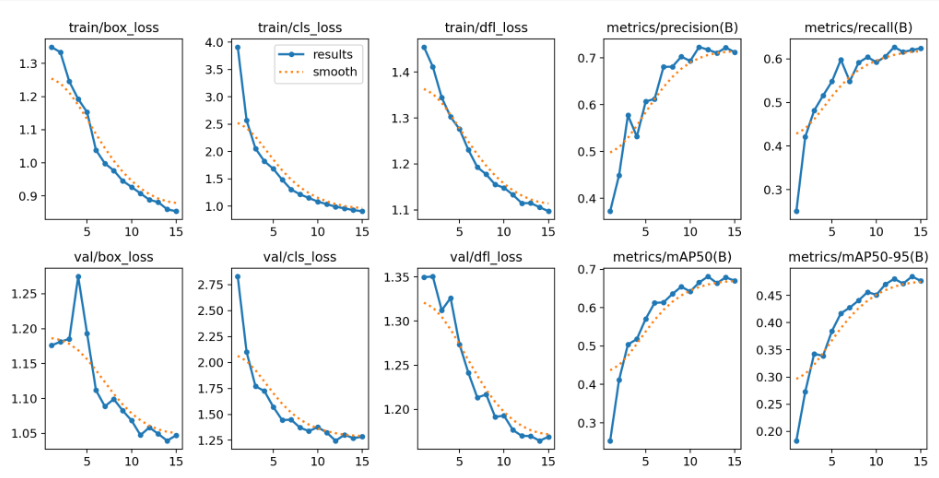
\includegraphics[width=0.5\textwidth]{4471_transfer_learning.png}
    \caption{Result of Transfer Learning}\label{transfer-learning-result}
\end{figure}
\begin{figure}[htbp]
    \centering
    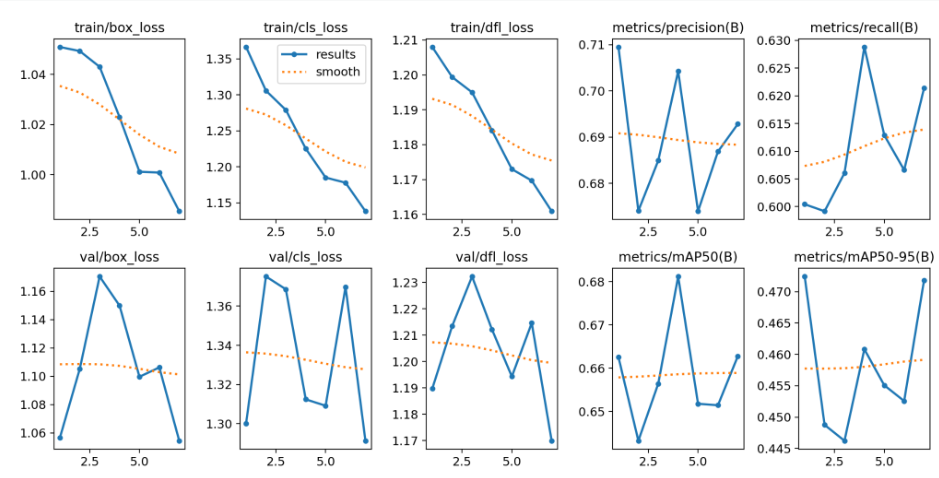
\includegraphics[width=0.5\textwidth]{4471_fine_tuning.png}
    \caption{Result of Fine Tuning}\label{fine-tuning-result}
\end{figure}

We also have studied confusion matrix after both transfer learning~\ref{transfer-learning-confusion} and fine tuning steps~\ref{fine-tuning-confusion}, analyzing what types of food are most commonly mistaken by the model.
Just as it was expected, most confusion was coming from treating food as some background objects.
It is especially clear in case of pineapples, we believe the problem stems from their unusual for food texture and green grass-like part.

\begin{figure}[htbp]
    \centering
    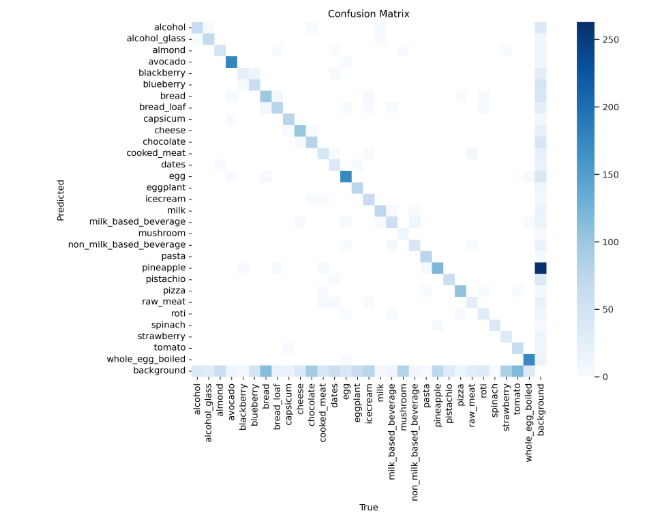
\includegraphics[width=0.5\textwidth]{4471_transfer_confusion.png}
    \caption{Confusion matrix of Transfer Learning}\label{transfer-learning-confusion}
\end{figure}
\begin{figure}[htbp]
    \centering
    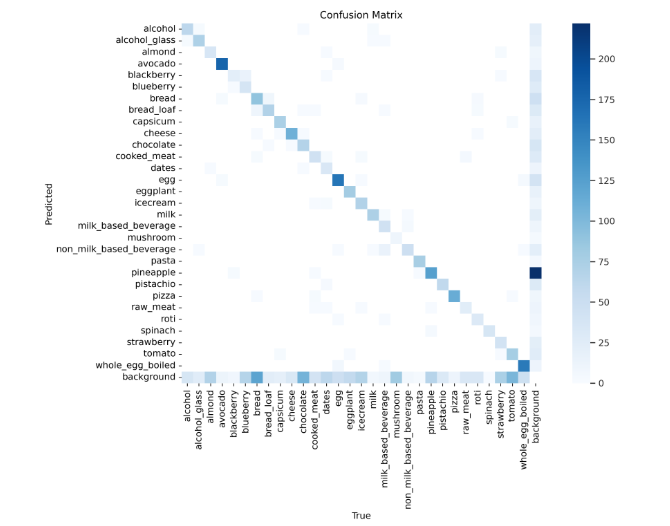
\includegraphics[width=0.5\textwidth]{4471_finetuning_confusion.png}
    \caption{Confusion matrix of Fine Tuning}\label{fine-tuning-confusion}
\end{figure}

From the above graphs, although the performance didn't improved a lot, there are an increase around $0.02$ which indicates the model has a small improvement (but actually precision decrease $0.015$). 
Overall, according to the the confusion matrix, the trained model perform quite well that most of the deep color (number of crossover between prediction and true label) are in the diagonal lines (predict correctly). 
The allergen detection task showed good results, with a precision of 0.707 and recall of 0.602 by the model.
These metrics show that the model is effective in correctly identifying allergenic foods while keeping a reasonable rate of false negatives.
The accuracy at a threshold of 50\% was 0.662, while accuracy between 50\% and 95\% was 0.472.
These results indicate that our model can differentiate between different food items, thus providing necessary alerts for users with food allergies.
So we are mostly satisified on the result~\ref{complete-detection-result-1}~\ref{complete-detection-result-2}~\ref{complete-detection-result-3}.

\begin{figure}[htbp]
    \centering
    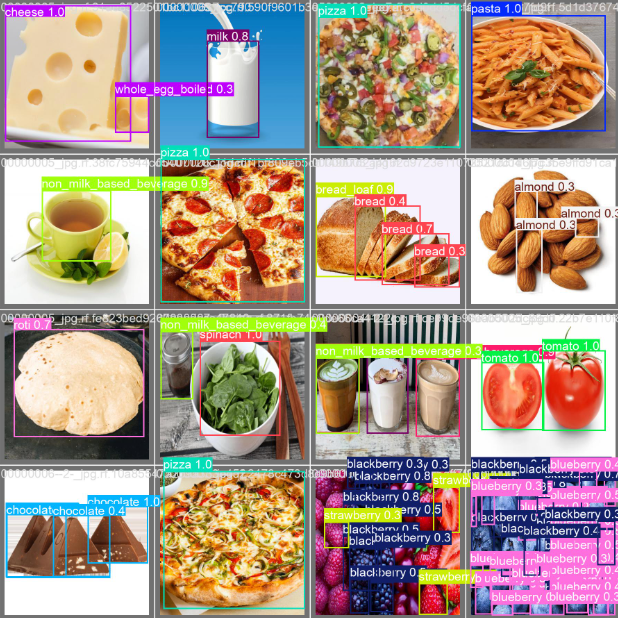
\includegraphics[width=0.5\textwidth]{detection-result-1.png}
    \caption{Result of the model}\label{complete-detection-result-1}
\end{figure}
\begin{figure}[htbp]
    \centering
    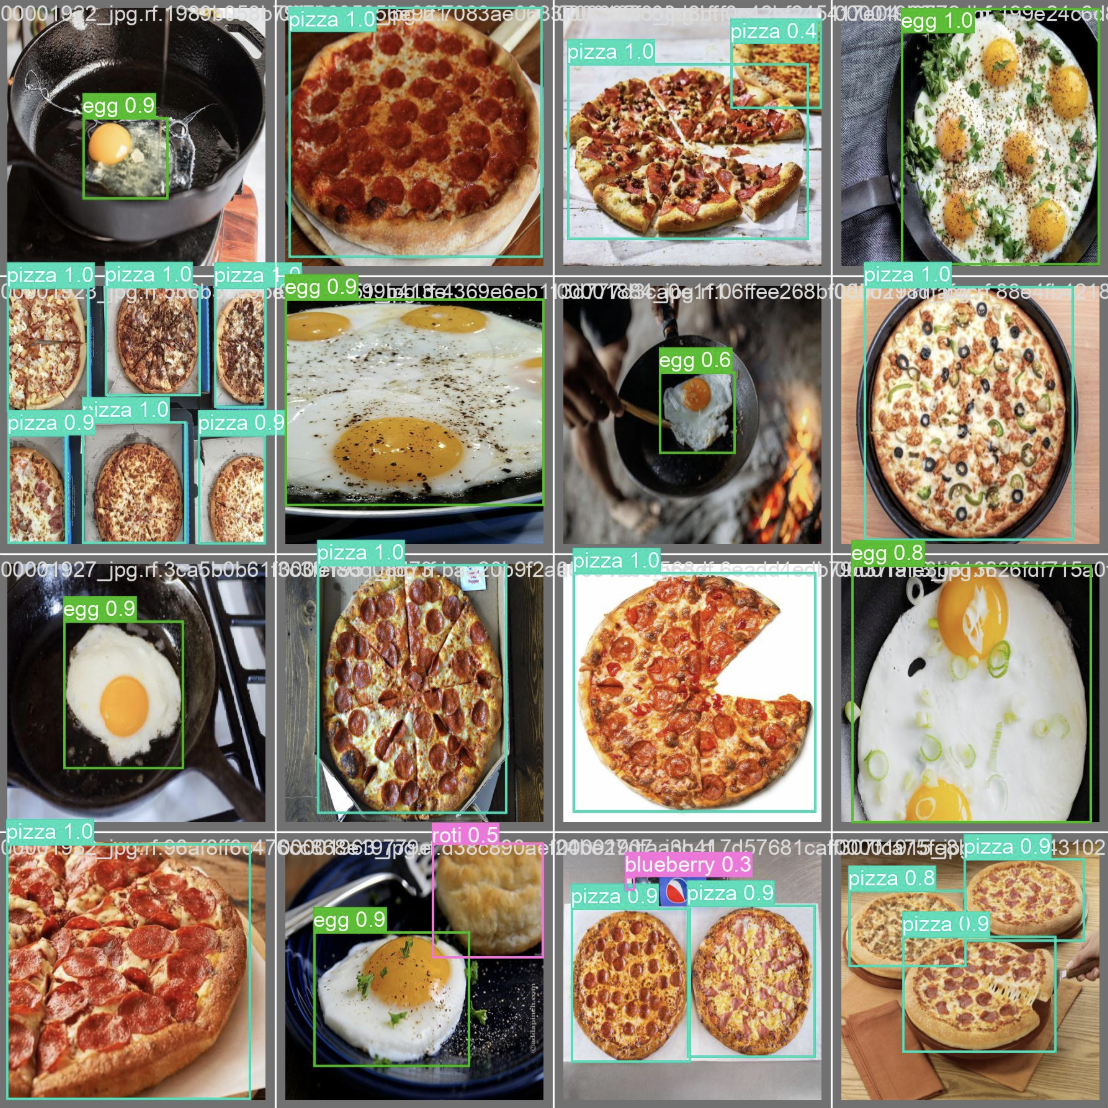
\includegraphics[width=0.5\textwidth]{detection-result-2.png}
    \caption{Result of the model}\label{complete-detection-result-2}
\end{figure}
\begin{figure}[htbp]
    \centering
    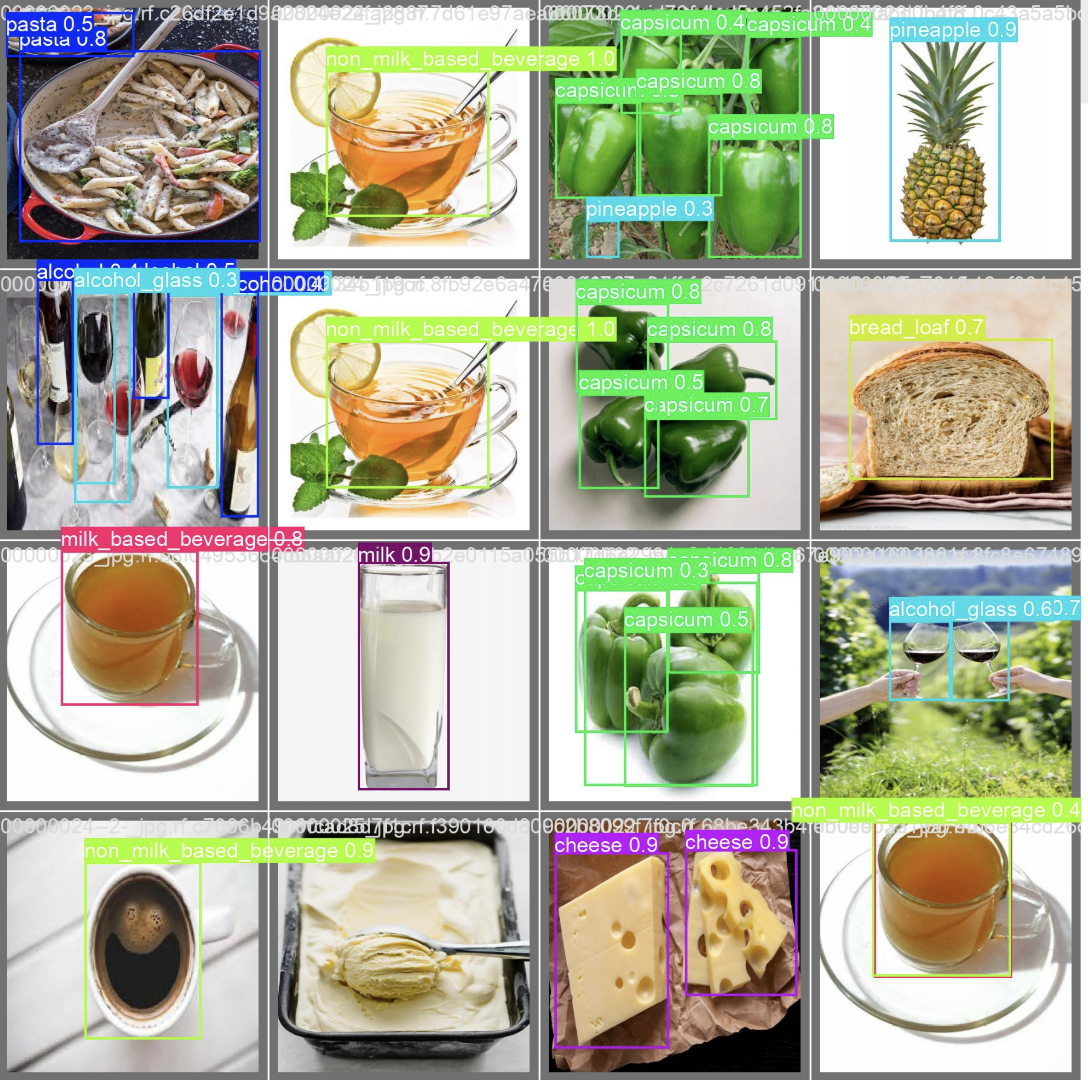
\includegraphics[width=0.5\textwidth]{detection-result-3.png}
    \caption{Result of the model}\label{complete-detection-result-3}
\end{figure}

As it was mentioned above, only for some of the food types calories amount estimation is available.
These food types are: avocado, dates, pineapple, capsicum, eggplant, spinach, tomato, milk, chocolate, pizza, egg, roti.
For now, the calories estimation algorithm includes just searching for the predicted food type in the database, loaded alongside with the model.

In order to provide our algorithm user with an insight on how could the model be used for a single image detection, a small client application using PyTorch library~\cite{torchlibrary} only was written in Python.
It accepts one single image, searches for food on it and returns a tuple containing found food object type, number of calories, confidence and predicted position in the image.
A screenshot~\ref{simple-client-result} shows the simple client output.

\begin{figure}[htbp]
    \centering
    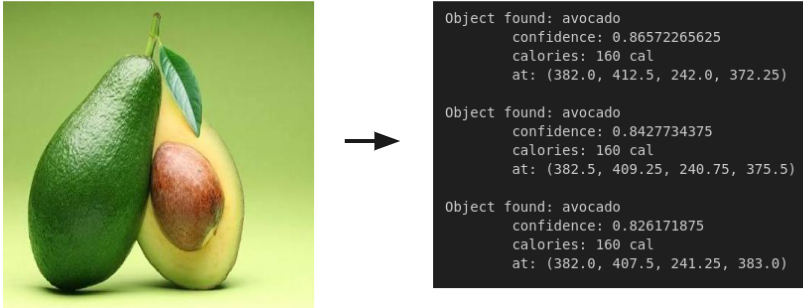
\includegraphics[width=0.5\textwidth]{simple-detector.png}
    \caption{Result of the model}\label{simple-client-result}
\end{figure}

JuPyter notebook that was used for training as well as the trained model will be submitted alongside with this report.
After training, model weights were published as \texttt{.pt} and \texttt{.onnx} files to the project repository~\cite{projectRepo} (together with the current report version).

Unfortunately, the results of our work up to this point are not easy to visualize for a non-professional.
Running a JuPyter notebook includes lots of initial setup, library version management, etc.
In order to make our project results more accessible for teh general public (as they are meant for everyday use), we have deployed an advanced client application: a website capable of evaluating the model as well as performing calories lookup.
The website is based on React framework and \texttt{onnxruntime-web} library.
Many of the machine-learning-related functions are not implemented in JavaScript, so we had to re-implement things such as tensor filtering or non-max suppression from the scratch.
The final result screenshot is included in this report~\ref{advanced-client-result} and the website can be found statically deployed on the project GitHub1~\cite{projectWebsite}.

\begin{figure}[htbp]
    \centering
    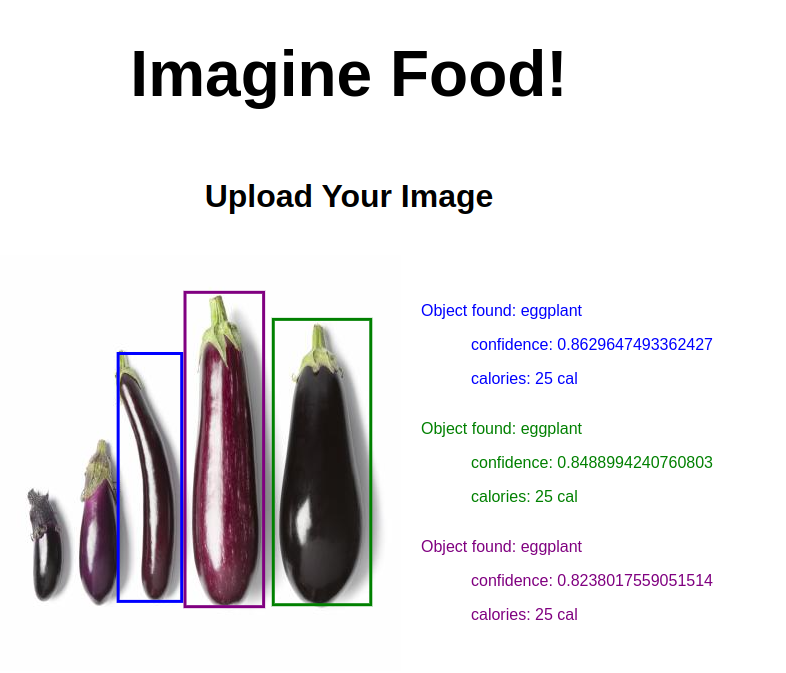
\includegraphics[width=0.5\textwidth]{advanced-detector.png}
    \caption{Result of the model}\label{advanced-client-result}
\end{figure}

\section{Conclusion}

This project has successfully shown the application of YOLOv11 in detecting and estimating calories and allergens in food item images. 
We have integrated transfer learning with the Allergen30 dataset to develop a model that identifies food items. 
Some formal results showing that we have good precision and recall means it can be used in real world.
The model now can estimate the calories and allergen of multiple food in an image to those health conscious users for reference with satisifed accuracy.
Based on what we learned we discovered that fine-tuning after transfer learning with pre-trained models improves both accuracy and speed significantly on complex tasks, in our case food recognition and allergen detection.
Moving from a traditional image classification to an object detection framework is beneficial as it allows to identify multiple food items within a single image.
This will not only simplify the requirements of the dataset but also improve the generalization of the model towards dietary patterns in diverse food presentations.

Our findings highlight the potential of using deep learning techniques in our daily life. 
In this project, we focus on nutrition, but the technique can be also used in other parts of our daily life.
For example, deep learning in computer vision could bring assist in medical image analysis for early detection and diagnosis in healthcare.
And the application of computer vision for pet monitoring systems can send alerts in case of any unusual activities, thus ensuring the pet's safety and well-being while assuring the owner.

Furthermore, there are several directions we can work on deeper in this project. 
One of the main points is the enrichment of the dataset. 
Currently, our model is able to estimate only a few types of food. 
By collecting more general and diverse food images, one can significantly enhance the capability of the model in recognizing and analyzing a wide variety of food. 
Moreover, we will be able to extend the nutritional analysis functionality. 
While currently our model focuses on calorie and allergen detection, it can be further trained to estimate other nutritional information like the content of proteins, vitamins, and minerals. 
Such a wide-range analysis will help users understand better to make conscious decisions regarding their health and nutrition.


%%%%%%%%% REFERENCES
{
    \small
    \bibliographystyle{bibliostyle}
    \bibliography{bibliography}
}

\end{document}
